\chapter{Method}
\label{chap:method}

% In this chapter, we discuss the methodology of the thesis. We motivate and specify the research question, state the hypothesis and the specify how we test it.

In this chapter, we introduce the methodology for experiments conducted in this thesis.

\section{Methodology overview}

Methodology

what do we want to measure? The effects of tokenization over the languages, focus on the differences the methods make on low resource vs high resource and how this translates to downstream tasks.b

- data sampling
    - !! do data hodně vysvětlit, že u toknizerů používáme různá alpha ale u pretrainingu ne.

- introduce the metrics
    - obecně naše metriky předpokládají nějaký předem daný vocabulary budget, který chceme spravedlivě rozdělit
    - CPT, AR, JSD
        - k AR metrice: je to samozřejmě závislý na vocab size, ale měl bych to poznamenat
        - výhoda AR oproti CPT - u čínštiny započítává jednotlivé znaky, což by u CPT nebylo vidět

        - k JSD metrice: není zřejmé jestli chceme vyšší overlap nebo nižší

    - interpretation of the metrics - CPT, AR high good, JSD not sure
    - also mention UNK and alphabet size
- kinds of experiments
    - tokenizers only
        - eg: training data size, alphabet size, data imbalance
    - tokenizers + MLM training
        - eg: Huggingface tokenizers, replications
    
- introduce the evaluation procedure
    - intrinsic evaluation
        - overall metrics - why macro average over languages
            - how to average JSD - all pairs
        - per language metrics - why delta from some baseline, metrics are different for different languages so we need to normalize
    - extrinsic evaluation
        - in-language / cross-language
            - overall - why macroaverage, per-language, how to do per-language in cross-lingual where there are pairs (we focus on target results)
            - seeds, averaging, bootstrapping
        - probing vs finetuningn
            - vysvětlit proč jsou všechny experimenty probing a jak se to liší a proč jsme to vybrali
        - tasks NLI, NER, POS tagging, ...
    - correlation between intrinsic and extrinsic
        - how to compute the correlation
        - míra korelace závisí na tom, jak moc se liší experimenty. Když porovnáváme jen stejné experimenty, pak nám vyjde nízká


Experiments
- data, languages - how did we select them
- vocabulary size - what did we pick, how does it relate to the previous work
- tokenizers replication
    - what are the variant we create
    - add the cluster assignment tables
    - přidat víc podrobností o našich replikacích - jaké clustery jsme dostali (Chung, Liang), jaké vocab sizes jsme alokovali (Zheng)

- Huggingface vs Sentencepiece
    - what are the parameters, how do we choose them or do we test them, what are the defaults
    - tokenizer training - memory requirements, time requirements   
- vanilla Unigram tokenizers
- TokMix

- maybe a table with all the tokenizers and their explanations

- training MLMs - technical details
    - machines
    - masked token ratio 15%

- probing MLMs - technical details
    - chosen tasks for each experiment, metrics for tasks
    

% - training the models
%     - we train with 10K steps, 8192 batch size, 128 sequence length
%     - on 2x A100
% - evaluation on downstream
%     - utilized Huggingface examples for the downstream tasks so that there are no mistakes
%     - on how to compute significance for the cross-lingual tasks
%         - we want to compare the average over languages
%         - we can use bootstrapping to compute the confidence intervals
%             - for each language select a random seed and compute the average over these seeds
%             - sample many times and compute the confidence intervals
% To be able to compare several tokenization methods we need to fix a training and evaluation procedure that we will use throught the thesis for each experiment, be it a replication of a previous work or our own novel method. In following sections we describe the training and evaluation procedure that we use in the thesis.

% For all experiments we use the CC100 dataset used in \citet{conneau_unsupervised_2020}. Using the data we create multilingual vocabularies with the same size of 120K unique tokens using different methods. We use intrinsic evaluation framework from \citet{limisiewicz_tokenization_2023} to evaluate the tokenizers. Then we use the tokenizers to train multilingual masked language models on the same data and evaluate them on the same set of downstream tasks. We compare the results of the intrinsic and extrinsic evaluation to see if the improvements in the intrinsic evaluation translate to improvements in the downstream tasks.

In this thesis, we investigate the effect of tokenizer properties on multilingual language models. We define metrics that measure the properties of the tokenizers and then we define the method by which we assess how these properties affect the performance of the language models. At the same time we want to improve the performance of the multilingual language model for the low-resource languages as this was shown to be a problem in previous work \cite{rust_how_2021}. Therefore we use the metrics we define to assess the methods proposed to solve this problem. Furthermore we propose methods to improve the performance of the language models and evaluate them using the same metrics.



\section{Data and scope}
\label{sec:data_scope}
% - prepare the pretraining/tokenizer training data
%     - selecting the dataset
%         - mBERT, Zheng - wikipedias
%         - XLM, Chung, Liang - CC100 
%     - select the languages
%         - which languages to use
%         - we follow the XNLI selection more or less
%         - show the table with the languages
%     - download the data
%         - how much data to use
%     - subsample the data
%         - what alphas to use?
%             - Conneau, Chung uses 0.3 \xxx{check this}
%             - Liang uses T=2 -> alpha=0.5
%             - Zheng uses 0.7!
%         - we choose alpha 0.0 and 0.3 (for Limi it was 0.25)
%         - we also create a evaluation and test set

For training the vocabularies and the masked language models we follow our related work \cite{conneau_unsupervised_2020,chung_improving_2020,liang_xlm-v_2023} and use the CC100 dataset. The other common choice is using Wikipedia data \cite{devlin_bert_2019,zheng_allocating_2021} but the CC100 have been shown to improve low-resource languages such as Swahili and Urdu \cite{conneau_unsupervised_2020}.

This unlabeled, multilingual dataset was created from the Common Crawl corpus using an automatic pipeline. The data was deduplicated and language-identified. Then for each monolingual corpus the data was filtered using Kneser-Ney language models trained on Wikipedia. Documents with perplexity under a certain language-specific threshold were filtered out. The data processing pipeline is described in detail in \citet{wenzek_ccnet_nodate}. A reproduction of the dataset is available at \url{https://data.statmt.org/cc-100/}.

For the purposes of this thesis, we select 20 out of 116 languages following \citet{limisiewicz_tokenization_2023} and download 10\% of the data for each language. The reason for selecting a subset of the languages available and using only part of the data is our computational constraints. First, by limiting the amount of data, we can train the models faster. Second, by limiting the number of languages, we can scale down the vocabulary size. Because a large amount of the model parameters is in the embedding matrix, the vocabulary size has a large impact on the model size. In turn this affects the training time and the memory requirements. We use the same 20 languages for all experiments in this thesis.

The exact choice of the language subset is motivated by the downstream evaluation datasets. We use the 15 languages covered by XNLI and add 5 more. The languages are selected to cover a wide range of language families and scripts. The full list of languages is shown in Table \xxx{tab:languages}.

\todo{add table with the languages with a summary of some of the properties (which languages share script, which are typologically related, which use spaces and which don't, which are low-resource)}

\begin{table}
    % uncomment the following line if you use the fitted top captions for tables
    % (see the \floatsetup[table] comments in `macros.tex`.
    %\floatbox{table}[\FBwidth]{
    \centering\footnotesize\sf
    \begin{tabular}{llrl}
    \toprule
    Language & Language code & Script \\
    \midrule
    English & en & Latin \\
    Vietnamese & vi & Latin \\
    Russian & ru & Cyrillic \\
    French & fr & Latin \\
    German & de & Latin \\
    Spanish & es & Latin \\
    Thai & th & Thai \\
    Bulgarian & bg & Cyrillic \\
    Hebrew & he & Hebrew \\
    Chinese-simplified & zh-Hans & Chinese \\
    Greek & el & Greek \\
    Turkish & tr & Latin \\
    Arabic & ar & Arabic \\
    Hindi & hi & Devanagari \\
    Tamil & ta & Tamil \\
    Georgian & ka & Georgian \\
    Urdu & ur & Arabic \\
    Telugu & te & Telugu \\
    Marathi & mr & Devanagari \\
    Swahili & sw & Latin \\
    % \addlinespace % a nice non-intrusive separator of data groups (or final table sums)
    \bottomrule
    \end{tabular}
    %}{  % uncomment if you use the \floatbox (as above), erase otherwise
    \caption{List of languages used in the experiments.}
    %}  % uncomment if you use the \floatbox
    \label{tab:languages}
\end{table}
    

% This subset of CC100 is then used for further experiments with vocabulary creation that will be described in the following sections.
\xxx{TODO: describe the resampling method, compare different alphas used in the literature}
For pretraining the models and training the tokenizers we do not use the full 10\% of the data. Because the data is heavily skewed towards the high-resource languages. Instead, we further subsample the data, following \citet{conneau_unsupervised_2020-1} to balance the number of lines per language. This is a standard practice followed by multiple independent authors \xxx{cite}. The empirical probability of sampling a line from language $l$ is given by:

\begin{equation}
    p(l) = \frac{N_l}{\sum_{l' \in L} N_{l'}}
\end{equation}

Where $N_l$ is the number of lines in the dataset for language $l$.

To ensure that the low-resource languages are not underrepresented in the training data, we modify this probability distribution using an exponential smoothing parameter $\alpha$:

\begin{equation}
    p'(l) = \frac{p(l)^\alpha}{\sum_{l' \in L} p(l')^\alpha}
\end{equation}

For $\alpha = 0$ we get the uniform distribution over the languages, for $\alpha = 1$ we get the original distribution. For pretraining the language models, we use $\alpha = 0.3$ as suggested by \citet{conneau_unsupervised_2020-1}. For training the tokenizers, we specify the alpha as a parameter of the tokenizer training procedure. Usually we use $\alpha = 0.0$ (1 milion lines per language, 20 milion in total) and $\alpha = 0.3$.

We also sample uniformly from the rest of the CC100 dataset to create evaluation and test splits. Here we use $\alpha = 0.0$ to represent all languages equally.

\section{Tokenizer metrics}

\xxx{lets write the motivation here and maybe move it to the background section later}  

% - motivation: we want to evaluate the tokenizers before costly pretraining
% - by comparing the tokenizers we can select the best one for pretraining
% - we can also use the metrics to study the effect of the hyperparameters and other factors on the tokenizer
% - We use the metrics throughout the thesis to measure the tokenizers
% - We can measure how the tokenizer output differs between languages
%     - Explain how to measure individual languages with the same tokenizer. Metric may be a function of the tokenizer and language coded hold out data

% - Why do we want to measure the tokenizers?
%     - we want to select the best tokenizer for pretraining
%     - how do the tokenizers differ?
%         - overlap between languages - can be beneficial for some tasks (ner) but detrimental for others (pos)
%         - how much do they split words? (Rust)
%         - how much do they split sentences? (Limisiewicz)
%             - too much splitting - the model needs to learn to reconstruct words
%             - too little splitting - there is not enough examples for the model to learn from (but maybe this is not a problem for masked LM, only for machine translation)
%         - we can also measure the compatiblity of the segmentations (Maronikolakis)
%         - vocabulary capacity per language
%             - are the languages represented equally in the vocabulary?
%             - this is hard because some languages need more tokens than others (Chinese vs English)

% - how to measure tokenizers
%     - we want to measure the per-language and cross-lingual phenomena
%     - we therefore need to measure the tokenizers using language-coded data
%     - the basis for measurement will be the tokenization of the language-coded data and the empirical distribution of the tokens

%     - Average Rank - we want to measure how many tokens are used in the vocabulary - high frequency tokens are penalized because they move the average down
%         - another motivation - AR is similar to "the number of tokens needed to cover x% of the data" but it is non-parametric and includes the information about the distribution of the tokens
%     - Characters per Token - more characters = less ambiguity = better
%         - similar to word fertility, equivalent to tokens per sentence
%             - tokens per sentence used in Chung (they call it description length), Liang
%         - usable also in the langugaes without spaces
%     - of course both measures depend on the langugage

%     - interesting: ALP === entropy * avg_sequence_length

%     - overlap - what is the overlap between two languages
%         - we can look at the number of tokens that are shared between the languages but this is not that informative because these tokens might be very rare
%             - Wu and Dredze did this
%         - better is to look at the distributions of the tokens in each language and measure the similarity
%         - we can use the Jensen-Shannon divergence to measure the similarity of the distributions
%         - Chung used the Wasserstein distance but this is a distance function defined between probability distributions on a given metric space. (probability measures). We do not see how to interpret the token distribution as a probability measure and Chung does not discuss this

In this section we introduce the metrics that we use to evaluate the tokenizers. By measuring the tokenizers we would like to explore two questions. First, we would like to analyse how the tokenizers differ between each other. How granular is the segmentation given an example text? And how much are the tokens shared between the languages? Second, using the observed differences between tokenizers, we would like to analyse how they influence the multilingual language models, that are trained using the tokenizers. We will describe the methodology for measuring the influences in the following sections \xxx{ref}.

When assessing the multilingual tokenizers, we also want to focus not only on the overall properties but also investigate the quality of tokenization for the individual languages. This gives us a better understanding of the tokenizers and allows us to compare the tokenizers between each other given a target language. For this purpose, we will use samples of evaluation corpora for each language. The metrics we define will be therefore functions of the tokenizer $\tau$ and the corpus $C_l$ with the selected language $l$. 

For each metric we will provide motivation and comparison with similar metrics used in the literature. 

\xxx{mention the vocabulary allocation and vocabulary overlap}
\xxx{TODO: add UNK rate?!}

\subsection{Characters per token}

\begin{figure}[h]
    \centering
    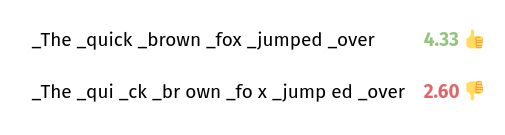
\includegraphics[width=0.6\textwidth]{img/temp/cpt_example.png}
    \caption{Example of CPT metric.}
    \label{fig:cpt_example}
\end{figure}

The first metric we will use is the average number of characters per token (CPT). The motivation for this metric is that we want to measure how granular the tokenization is. If the tokenizer splits the words into many tokens, the average number of characters per token will be low. On the other hand, if the tokenizer does not split the words, the average number of characters per token will be high. We hypothesize, that longer tokens are better for the language models, because they potentially carry more meaning. The extreme case of this metric is the character-level tokenization, where the average number of characters per token is 1. In this case the model would need to learn to reconstruct the words from the characters.

The metric is defined as follows. Given a tokenizer $\tau$ and a language corpus $C_l$, we first tokenize the corpus using the tokenizer $\tau$. Then we compute the average number of characters per token in the tokenized corpus:

\begin{equation}
    CPT(\tau, C_l) = \frac{\sum_{s \in C_l}|s|}{\sum_{s \in C_l}|\tau(s)|}
\end{equation}

where $|s|$ is the number of characters in the sentence $s \in C_l$ and $|\tau(s)|$ is the number of tokens in the tokenized sentence. The metric is illustrated in Figure \ref{fig:cpt_example}.

\subsection{Average Rank}

\begin{figure}[h]
    \centering
    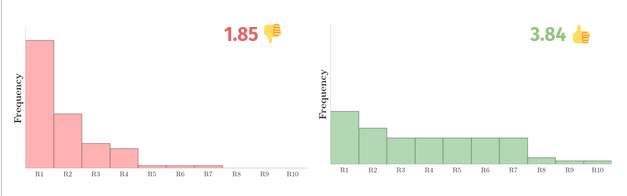
\includegraphics[width=0.6\textwidth]{img/temp/ar_example.png}
    \caption{Example of AR metric.}
    \label{fig:ar_example}
\end{figure}

Another metric we use for comparing the tokenizers is Average Rank (AR). The motivation for this metric is that we want to measure how many tokens are effectively used in the vocabulary for representing the corpus. Each language will have some amount of tokens dedicated to it in the vocabulary and our goal is to measure this allocation. We also want to take into account how frequently are these tokens used. We hypothesize that very frequent and very rare tokens are not as useful for the language models as the high-frequency tokens might be too ambiguous and low-frequency tokens might not have enough training examples to learn from \cite{gowda_finding_2020}. We therefore propose to measure the average rank (the position of the token sorted by frequency) of tokens needed to cover a monolingual corpus, weighted by their probability.
% Here one metric suggestion could be something along the lines of "number of tokens from vocabulary of $\tau$ needed to cover the 95/98/100\% of the corpus". That metric would work but the downside is that we do not know how to set the threshold. Moreover we would like the metric to reflect the shape of the distribution of the token coverage. We prefer a distribution that is more balanced. High-frequency tokens might be too ambiguous and low-frequency tokens might not have enough training examples to learn from \cite{gowda_finding_2020}. Therefore we propose a different metric that reflects both the vocabulary allocation and the uniformity of the token distribution. On top of that it is parameter-free.

Given a tokenizer $\tau$ and a language corpus $C_l$, we first tokenize the corpus using the tokenizer $\tau$. Then we compute the empirical probability of the tokens in the tokenized corpus.

\begin{equation}
    \hat{p}_{\tau(C_l)}(t) = \frac{count(t, \tau(C_l))}{\sum_{t' \in \tau(C_l)} count(t', \tau(C_l))}
\end{equation}

We sort the tokens by their probability and assign them ranks from 1 to $|V_\tau|$. The average rank is then the weighted average of the ranks of the tokens, where the weights are the probabilites of the tokens:

\begin{equation}
    AR(\tau, C_l) = \sum_{t \in V_\tau} rank(t, \tau(C_l)) \cdot \hat{p}_{\tau(C_l)}(t)
\end{equation}

The metric is illustrated in Figure \ref{fig:ar_example}. Higher AR signals that the vocabulary contains higher number of tokens used for tokenizing given language. Moreover with high AR we can expect that the tokens are distributed more uniformly.

\subsection{Jensen-Shannon Divergence}

\begin{figure}[h]
    \centering
    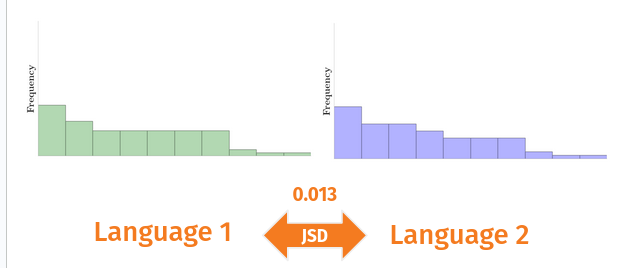
\includegraphics[width=0.5\textwidth]{img/temp/jsd_example.png}
    \caption{Jensen-Shannon Divergence}
    \label{fig:jsd_example}
\end{figure}

The Jensen-Shannon Divergence (JSD) is a metric that measures the similarity between two probability distributions. It is defined as follows:

\begin{equation}
    JSD(p, q) = \frac{1}{2} \cdot (KL(p||m) + KL(q||m))
\end{equation}

Where $m = \frac{1}{2} \cdot (p + q)$ is the midpoint distribution and $KL(p||q)$ is the Kullback-Leibler divergence. 

\begin{equation}
    KL(p||q) = \sum_{t \in V_\tau} p(t) \log \frac{p(t)}{q(t)}
\end{equation}

We will use JSD for the analysis of an overlap between two languages given a tokenizer. Tokenization of two monolingual corpora $C_{l_1}$ and $C_{l_2}$ with the same tokenizer $\tau$ will result in two probability distributions over the vocabulary $V_\tau$. We will denote these distributions as $\hat{p}_{\tau(C_{l_1})}$ and $\hat{p}_{\tau(C_{l_2})}$. 

Computing the JSD between the two distributions will result in a metric that measures how much the two distributions overlap. The JSD is a symmetric metric that is bounded between 0 and 1. Low JSD means that the two distributions are similar, high JSD means that the two distributions are different. 

% Further, we will be mainly concerned with the tokenization of the training corpora $\tau(C_l)$ and the empirical distribution over the tokenizer vocabulary:

% \xxx{fix the equation once I settle on the notation. The denominator is wrong here}

% - test the tokenizer metrics, show correlation between CPT, AR and JSD -> downstream
%     - define the metricshe implementation}

% In \cite{limisiewicz_tokenization_2023} we have compared the Unigram LM and BPE tokenizers. We have found that generally, the BPE tokenizer performs better on the tokenizer intrinsic metrics and the downstream tasks. During the work on the thesis we have found that this finding might have been heavily influenced by the choice of the implementation of the Unigram LM training algorithm. In \cite{limisiewicz_tokenization_2023} we have used the Huggingface implementation of the tokenizers. In the later experiments we have used the Sentencepiece implementation. We have found that the Sentencepiece implementation produces tokenizers that close the gap in the intrinsic evaluation. We have therefore decided to use the Sentencepiece implementation for all experiments in this thesis.

% \xxx{add image}

% \xxx{TODO: add the other factors - co
%         - CPT
%         - AR
%         - JSD
%     - compare 4 tokenizers
%         - vanilla Unigram, vanilla BPE
%         - NoOverlap - to study the effect of the overlap
%         - TokMix - to ensure a uniform 
%     - experiments for 6 languages
%     - experiments for 20 languages

% \section{Investigating the influence of the tokenizer on the language model}

\section{Extrinsinc evaluation}

\tomasz{Here, I would write section Extrinsic Evaluation. 
With general description assesing tokenizer influnce on downstream tasks.
Details should be provided in the next chapter: Experiments...}

